%# -*- coding: utf-8-unix -*-
%%==================================================
%% 03_zuc.tex % 2.5k
%%==================================================

\chapter{ZUC 算法的软硬件实现}

\label{chap:zuc}

\section{算法背景} % 0.5k
% 《3GPP LTE 国际加密标准 ZUC 算法》
祖冲之算法,又称 ZUC 算法,是我国提出的第一个国际商用标准密码算法。

2004 年,3GPP(3rd Generation Partnership Project,第三代合作伙伴计划)提出了 LTE(Long Term Evolution,长期演进),目的是保证该计划能够继续在电信行业拥有一定的话语权。在 2010 年底,3GPP 被确立为第四代(4G)移动通信标准。 \cite{lte}

安全性是通信技术中一个非常重要的指标,而密码算法又是保障安全性的一个重要工具。3GPP 之前已经拥有的两个算法是 AES 和 SNOW 3G,而 ZUC 算法则是第三个被纳入标准的算法。ZUC 算法的提出和设计历经了很多挑战,因为商用密码算法的要求非常严苛,既要保证极高的安全性,又要拥有较高地运行性能,还需要在各自环境下都方便实现。中国科学院等单位克服了重重困难,最终研制成功,经由中国通信标准化协会与工信部向 3GPP 组织提交了这一算法,并且经过了行业严格的评审,最终被批准成为 LTE 中的密码算法标准,参与到实际的商业应用。 \cite{zuc_test}

总之,ZUC 算法的提出,使我国在国际商用密码领域拥有了更多的自主权,既体现了我国在密码学领域的学术能力,又是我国参与制定国际化通信标准的重要一步。因此,研究 ZUC 算法,具有很高的现实意义。

\section{算法流程}
\label{sec:algoflow}

ZUC 算法分成三层,如下: \cite{zuc_standard}

\begin{itemize}
    \item \textbf{线性反馈移位寄存器(Linear feedback shift register,LFSR):}LFSR 有两种模式,初始化模式和工作模式。
    \item \textbf{比特重组(Bit Reorgnization, BR):}该层将寄存器中特定位置的数据进行编排然后输出。
    \item \textbf{非线性函数(Nonlinear Function, F):}这一层涉及到一个 S 盒置换,而 S 盒置换是非线性的,因此也是这个算法中非常关键的部分。我们后续的功耗分析攻击,将会重点关注这一部分。
\end{itemize}

\vspace*{0.5\baselineskip}

ZUC 算法的运行过程如下:\cite{zuc_standard}

\begin{enumerate}
    \item \textbf{初始化阶段:}这一部分包括初始密钥的装载,LFSR 和寄存器的初始化,以及重复 32 轮的打乱操作(每一轮都包含比特重组、非线性函数以及以初始模式运行一次 LFSR)。
    \item \textbf{工作阶段:}这一部分包括一个一次性操作(比特重组、非线性函数以及以工作模式运行一次 LFSR)以及密钥生成阶段(每一次密钥输出都包含比特重组、非线性函数、输出密钥以及以工作模式运行一次 LFSR)。
\end{enumerate}

\vspace*{0.5\baselineskip}

由于密码本身相对比较复杂,这里只是粗略地介绍了一下算法的基本组成部分和大致流程。我们在 \ref{sec:software} 节将会讨论关于算法的更多细节,另外也可以参考文献 \parencite{zuc_standard}。

作为攻击者和研究人员,了解算法的全部细节和设计理由固然重要,但是更加重要的是找到算法在实际实现中可能存在的问题。设计者和攻击者考虑问题的角度是不一样的,设计者往往拥有更好的大局观,但在细节上往往无法挖掘太深,而攻击者只需要撬动整个系统中的某一点就足以达成目标了。

因此我们将在下一节讨论对 ZUC 算法实施差分功耗攻击的方法。

\vspace*{0.5\baselineskip}

图 \ref{fig:zuc_algo} 展示了 ZUC 算法的过程。

\begin{figure}[htbp]
    \centering
    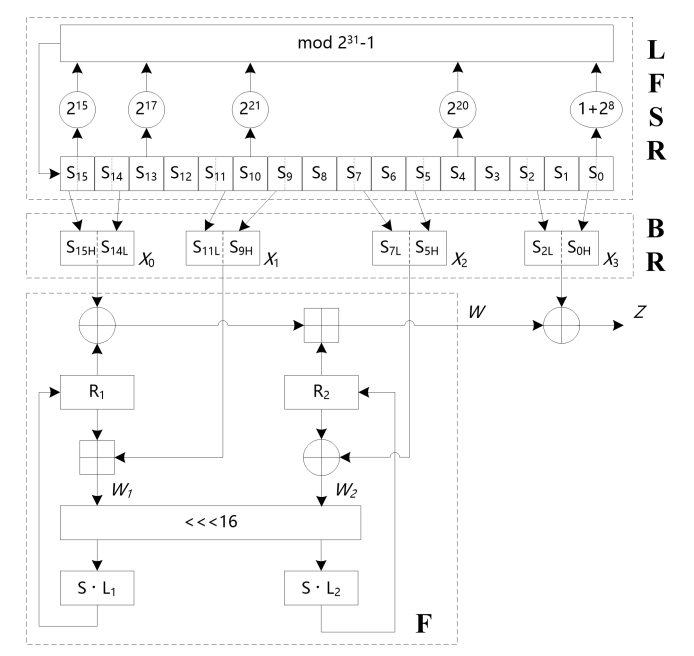
\includegraphics[height=.5\textheight]{../images/zuc_algo.png}
    \caption{ZUC 算法的流程图 \cite{zuc_standard}}
    \label{fig:zuc_algo}
\end{figure}


\section{硬件实现}
\label{sec:hardware}

硬件设计使用的软件是 ISE 14.3,使用的 FPGA 型号为:XC6SLX75-2CSG484。在完成硬件设计、仿真和综合后,在实际环境中运行 ZUC 算法,并采集功耗曲线,用于后续的分析。

这部分的代码实现和 \ref{sec:software} 节中所述的基本相同,但因为软件层面的代码可读性更强,因此我们将具体的实现细节留在 \ref{sec:software} 中详细阐述。

\newpage

硬件电路的输入和输出端口如图 \ref{fig:circuit_io} 所示。

\begin{figure}[htbp]
    \centering
    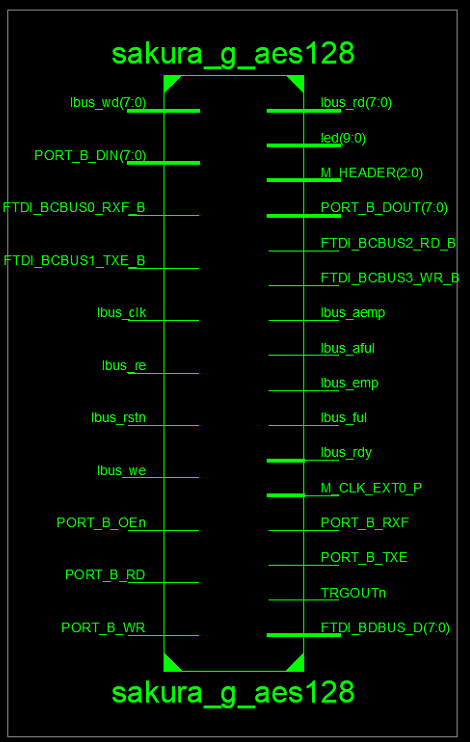
\includegraphics[height=.6\textheight]{../images/circuit_io.png}
    \caption{硬件电路的输入和输出端口}
    \label{fig:circuit_io}
\end{figure}

\newpage

硬件电路的内部结构如图 \ref{fig:circuit_more} 所示。

\begin{figure}[htbp]
    \centering
    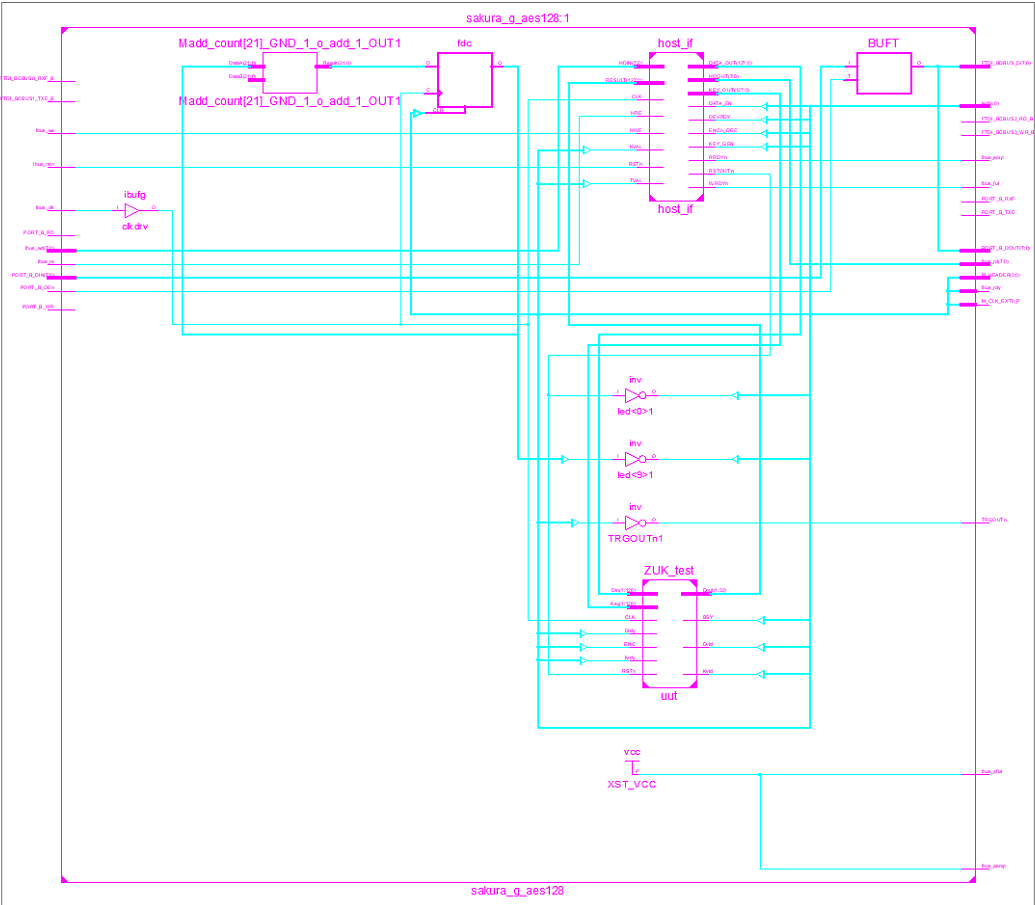
\includegraphics[height=.6\textheight]{../images/circuit_more.png}
    \caption{硬件电路的内部结构}
    \label{fig:circuit_more}
\end{figure}

\newpage

\section{软件实现}
\label{sec:software}

软件实现使用的语言为 Python 3.6,运行平台为 Windows 10。软件部分的作用是在功耗分析过程中计算中间值以及对应的假设功耗值,并进行相关系数攻击和更多的处理。软件代码开源在本人的 GitHub 仓库中:https://github.com/Hansimov/zuc-attack。

下面对软件实现的一些重要模块进行说明,作为对 \ref{sec:algoflow} 节的补充。

\subsection{符号和函数说明}
为了方便讨论,这里的符号基本保持和文献 \parencite{zuc_standard} 中的一致。

\begin{table}[htbp]
\caption{ZUC 算法中符号的说明}
\label{table:symbol}
\begin{tabular}{R{0.35\textwidth} L{0.65\textwidth}}
{\cnsls s[0] ,s[1], ..., s[15]} & 线性反馈移位寄存器模块的 16 个 31 比特寄存器单元变量 \\
{\cnsls x[0], x[1], x[2], x[3]}  & 比特重组模块输出的 4 个 32 比特字 \\
{\cnsls r1, r2} & 非线性函数模块中的 2 个 32 比特记忆单元变量 \\
{\cnsls w} & 非线性函数模块输出的 32 比特字 \\
{\cnsls w1} & r1 与 x[1] 进行模 $2^{32}$ 加法运算输出的 32 比特字 \\
{\cnsls w2} & r2 与 x[2] 按比特位逐位异或运算输出的 32 比特字 \\
{\cnsls z} & 算法每拍输出的 32 比特密钥字 \\
{\cnsls k} & 初始种子密钥 \\
{\cnsls v} & 初始向量,可以视为输入的明文 \\
{\cnsls d[0], d[1], ..., d[15]}  & 给定的 16 个 15 比特的字符串常量 \\
\end{tabular}

\end{table}

\begin{table}[htbp]
\caption{ZUC 算法中函数的说明}
\label{table:function}
\begin{tabular}{R{0.35\textwidth} L{0.65\textwidth}}
{\cnsls lsfrInit} & 线性反馈移位寄存器模块的初始化模式 \\
{\cnsls lfsrWork} & 线性反馈移位寄存器模块的工作模式 \\
{\cnsls nonLinearFunction} & 非线性函数模块 \\
{\cnsls linearTransform} & 非线性函数模块中的线性变换函数 \\
{\cnsls sboxOfZuc} & 非线性函数模块中的 S 盒置换函数 \\
{\cnsls bitReorganization} & 比特重组模块 \\
{\cnsls varsInit} & 所有变量初始化 \\
{\cnsls zucInit} & 算法运行的初始化阶段 \\
{\cnsls zucWork} & 算法运行的工作阶段 \\
{\cnsls outputkey} & 密钥输出 \\
\end{tabular}

\end{table}


\subsection{三层模块}

\subsubsection{线性反馈移位寄存器模块}

线性反馈移位寄存器模块拥有两个模式,分别是初始化模式和工作模式,二者唯一的区别在于\ {\cnsls s[16]} 的赋值方式。其中用到了素域上的模 $2^{31}-1$ 加法,需要具备一些抽象代数的基础知识。这部分的主要操作就是不断打乱和混淆寄存器中存储的变量。

该模块中的素域 $GF(2^{31}-1)$ 上的本原序列可以视为二元域 $GF(2)$ 上的非线性序列,具备一系列优点,比如线性复杂度高、随机性强、权位序列平移等价以及可以一定程度上抵抗现有的基于二元域的密码分析(区分攻击、相关攻击和代数攻击)。 \cite{zuc_feng}

\begin{lstlisting}[style=myPython,label={lst:lfsr},caption={线性反馈移位寄存器的初始化模式和工作模式}]
def lfsrInit():
    global k_hex, k, v_hex, v, d, s, w
    shift_bits_list  = [15, 17, 21, 20, 8, 0]
    shift_index_list = [15, 13, 10, 4, 0, 0]
    xv = [0] * 31
    for i in range(0, len(shift_bits_list)):
        s_i_shifted = circShiftLeft(s[shift_index_list[i]], shift_bits_list[i])
        xv = modAdd_2e31m1(xv, s_i_shifted)
    s[16] = modAdd_2e31m1(shiftLeft(w, -1), xv) # The only diffrence of lfsrWork() and lfsrInit()
    if s[16] == [0]*31:
        s[16] = [1]*31
    for i in range(0,16):
        s[i] = s[i+1]

def lfsrWork():
    global k_hex, k, v_hex, v, d, s
    shift_bits_list =  [15, 17, 21, 20, 8, 0]
    shift_index_list = [15, 13, 10, 4, 0, 0]
    xv = [0] * 31
    for i in range(0, len(shift_bits_list)):
        s_i_shifted = circShiftLeft(s[shift_index_list[i]], shift_bits_list[i])
        xv = modAdd_2e31m1(xv, s_i_shifted)
    s[16] = xv # The only diffrence of lfsrWork() and lfsrInit()
    if s[16] == [0]*31:
        s[16] = [1]*31
    for i in range(0,16):
        s[i] = s[i+1]
\end{lstlisting}

\subsubsection{比特重组模块}

比特重组模块的实现最为简单,其操作基本就是字符串的剪切和粘贴,建立起了上一层线性反馈移位寄存器和下一层非线性函数之间的桥梁。

简单的设计使这一模块便于在软硬件上实现,其作用是改变线性反馈移位寄存器部分的线性结构,并且加强对素域 $GF(2^{31}-1)$ 上密码分析的防御能力。 \cite{zuc_feng}

\begin{lstlisting}[style=myPython,label={lst:bitreorganization},caption={比特重组}]
def bitReorganization():
    global x, s
    x[0] = s[15][0:16] + s[14][-16:]
    x[1] = s[11][-16:] + s[9][0:16]
    x[2] = s[7][-16:] + s[5][0:16]
    x[3] = s[2][-16:] + s[0][0:16]
\end{lstlisting}


\subsubsection{非线性函数模块}
非线性函数模块的实现相对复杂一些,其中的 S 盒置换函数和分组密码的设计思想很相似。其中的操作较多,包括比特加、比特异或、模 $2^{32}$ 加、字符串移位以及 S 盒置换。

这一模块中的复杂运算和操作,从根本上改变了源序列在素域 $GF(2^{31}-1)$ 上的线性代数结构,而精心设计的 S 盒则具备很强的非线性性和扩散性。因此这一模块使整个算法的安全性得到了极大地提升。

\begin{lstlisting}[style=myPython,label={lst:nonlinearfunction},caption={非线性函数}]
def nonLinearFunction():
    global w, x, r1, r2
    w = binaryAdd(binaryXor(x[0], r1), r2)
    w1 = binaryAdd(r1, x[1])
    w2 = binaryXor(r2, x[2])
    r1 = sboxOfZuc(linearTransform(w1[-16:]+w2[0:16], 1))
    r2 = sboxOfZuc(linearTransform(w2[-16:]+w1[0:16], 2))
\end{lstlisting}

\vspace*{0.5\baselineskip}
非线性函数模块中有两个重要的函数:{\cnsls linearTransform} 和 {\cnsls sboxOfZuc}。

线性变换函数 { \cnsls linearTransform} 主要是将字符串的不同部分进行移位和比特异或。

\begin{lstlisting}[style=myPython,label={lst:lineartransform},caption={线性变换函数}]
def linearTransform(list_in, typex):
    if typex == 1:
        shift_bits_list = [0, 2, 10, 18, 24]
    else:
        shift_bits_list = [0, 8, 14, 22, 30]

    list_out = [0] * len(list_in)
    for i in range(0, len(shift_bits_list)):
        list_out = binaryXor(list_out, circShiftLeft(list_in, shift_bits_list[i]))

    return list_out
\end{lstlisting}

S 盒置换函数 { \cnsls sboxOfZuc} 主要是提供非线性性,将每个输入的字节映射到另一个截然不同的字节,其核心是两张 S 盒置换表。限于篇幅,这里没有将 S 盒中的所有元素都写出来。

\begin{lstlisting}[style=myPython,label={lst:sboxofzuc},caption={S 盒置换函数}]
def sboxOfZuc(list_in):
    sbox = [[]] * 4
    sbox[0] = [
        ['3E', '72', '5B', '47', 'CA', 'E0', '00', '33', '04', 'D1', '54', '98', '09', 'B9', '6D', 'CB'], 
        ...
        ]; # 16x16 list
    sbox[1] = [
        ['55', 'C2', '63', '71', '3B', 'C8', '47', '86', '9F', '3C', 'DA', '5B', '29', 'AA', 'FD', '77'], 
        ...
        ];  # 16x16 list
    sbox[2] = sbox[0]
    sbox[3] = sbox[1]
    list_out = [0] * 32

    for i in range(0, 4):
        list_tmp = list_in[8*i:8*(i+1)]
        hex_tmp = binvec2hex(list_tmp)
        row_tmp, col_tmp = hex2dec(hex_tmp[0]), hex2dec(hex_tmp[1])
        hex_tmp_s = sbox[i][row_tmp][col_tmp]
        list_out[8*i:8*(i+1)] = hex2binvec(hex_tmp_s)
    return list_out
\end{lstlisting}


\subsection{运行过程}

\subsubsection{变量初始化}

变量初始化部分就是给算法中要用到的变量赋初值,其中就包括将初始密钥装入寄存器的操作。

\begin{lstlisting}[style=myPython,label={lst:varsinit},caption={变量初始化}]
k_hex = [''] * 16
v_hex = [''] * 16
k = [''] * 16 # initial key     -  8 bit x 16
v = [''] * 16 # initial vector  -  8 bit x 16
d = [''] * 16 # constant data   - 15 bit x 16
s = [[0]*31 for _ in range(17)] # combined bit list - 31 bit x 16+1 (The last is used to update)
r1 = [0] * 32 # register 1 - 32 bit
r2 = [0] * 32 # register 2 - 32 bit
x = [[0]*32 for _ in range(4)] # list - 32 bit x 4
w = [0] * 32 # var in nonLinearFucntion(), used by zucInit()
d = [ '100010011010111', '010011010111100', '110001001101011', '001001101011110',
      '101011110001001', '011010111100010', '111000100110101', '000100110101111',
      '100110101111000', '010111100010011', '110101111000100', '001101011110001',
      '101111000100110', '011110001001101', '111100010011010', '100011110101100']

def varsInit():
    global k_hex, k, v_hex, v, d, s, r1, r2
    k_hex = ['00','00','00','00','00','00','00','00','00','00','00','00','00','00','00','00']
    for i in range(0, 16):
        k[i] = hex2binstr(k_hex[i])

    v_hex = ['00','00','00','00','00','00','00','00','00','00','00','00','00','00','00','00']
    for i in range(0, 16):
        v[i] = hex2binstr(v_hex[i])

    for i in range(0, 16):
        s[i] = k[i] + d[i] + v[i]
        s[i] = list(map(int,s[i]))
    r1 = [0] * 32
    r2 = [0] * 32

\end{lstlisting}

\subsubsection{算法运行}
算法运行分为两个阶段,分为初始化阶段和工作阶段。唯一的不同就是,初始化阶段执行的次数是固定的 32 轮,而工作阶段的执行次数取决于要输出多少次密钥。

算法运行过程中,需要不断地执行上一小节中提及的三个模块。

\begin{lstlisting}[style=myPython,label={lst:zuc},caption={算法初始化阶段和工作阶段}]
def zucInit():
    global k_hex, k, v_hex, v, d, s, r1, r2, x, w
    for i in range(0,32):
        bitReorganization()
        nonLinearFunction()
        lfsrInit()

def zucWork(i=0):
    global k_hex, k, v_hex, v, d, s, r1, r2, x, w
    bitReorganization()
    nonLinearFunction()
    key_bin = binaryXor(w, x[3])
    key_hex = binvec2hex(key_bin)
    if i != 0:
        print('Key {:>02} {}'.format(i, key_hex.lower()))
    lfsrWork()
\end{lstlisting}

\subsubsection{密钥输出}

这一部分非常简单,其核心就是进入整个算法的工作阶段,然后不断循环,输出密钥。

\begin{lstlisting}[style=myPython,label={lst:outputkey},caption={算法初始化阶段和工作阶段}]
def outputKey(num=1):
    global k_hex, k, v_hex, v, d, s, r1, r2, x, w
    for i in range(0, num+1):
        zucWork(i)
\end{lstlisting}

\subsubsection{运行结果}
运行如下代码,则会输出 3 次密钥。虽然工作阶段实际运行了 4 次,但是算法规定第 0 次输出的密钥要舍弃。

\begin{lstlisting}[style=myPython,label={lst:run},caption={完整的算法执行过程}]
if __name__ == '__main__':
    varsInit()
    zucInit()
    outputKey(4)
\end{lstlisting}

上述代码中,种子密钥和初始向量都是全 0 序列。

算法运行产生的输出如下:

\begin{lstlisting}[style=myPython,label={lst:runresult},caption={算法运行的输出结果}]
Key 01 27bede74
Key 02 018082da
Key 03 87d4e5b6
Key 04 9f18bf66
\end{lstlisting}

\section{本章小结}

本章首先讨论了 ZUC 算法的提出背景,介绍了其和通信行业发展的密切联系,并且指出了该算法对我国的重要意义。

然后我们讨论了 ZUC 算法的流程和结构,分别介绍了 ZUC 算法的三个部分,包括线性移位反馈寄存器、比特重组和非线性函数,并且讲解了初始化和工作的运行过程。

接着我们展示了 ZUC 算法的硬件实现情况和所用设备,给出了硬件电路的原理图。

最后我们详细讲解了算法的软件实现,分析了各个模块的操作和作用,这是我们后续对算法进行攻击的基础工作。


